\documentclass[runningheads]{llncs}
\usepackage[T1]{fontenc}
\usepackage{graphicx}
\usepackage{booktabs}      % professional tables (\toprule/\midrule/\bottomrule)
\usepackage{multirow}
\usepackage{amsmath,amssymb}
\usepackage{hyperref}
\renewcommand\UrlFont{\color{blue}\rmfamily}\urlstyle{rm}

% =====================================================================
%  WRITING NOTES (delete before submission)
%  - CONTENT (numbers, method, findings): ../FINDINGS.md, ../FINDING_1.md,
%    ../FINDING_2.md, ../FINDING_4.md, ../RESULTS.md  (authoritative — never invent a number).
%  - STYLE: Cambodia/WRITING_STYLE.md + the exemplar PDFs it points to.
%  - Figure 1 = ../figures/crossover_sparsity.pdf . Tables below are pre-filled with final numbers.
%  - Scope: CF vs LLM only. NO vision/CLIP (that is a separate paper; see ../FINDING_3.md).
%  - Honest limitations to keep: 1 seed, n=4 for the density law, 20 candidates, the Prime Pantry
%    Hit@5/10 nuance.
% =====================================================================

\begin{document}

\title{When Do LLMs Help Sequential Recommendation?\\
A Collaborative-Filtering$\leftrightarrow$LLM Complementarity Analysis}
\titlerunning{When Do LLMs Help Sequential Recommendation?}

% TODO(authors): fill in / anonymize for double-blind submission if required.
\author{Anonymous Author(s)}
\authorrunning{Anonymous}
\institute{TODO Institution}

\maketitle

\begin{abstract}
% First-pass draft (~180 words) — refine in the writing pass.
Large language models (LLMs) are increasingly bolted onto sequential recommenders, but it is unclear
\emph{when} they help. Using A-LLMRec---a frozen collaborative-filtering recommender (SASRec) aligned
with a frozen LLM---as an instrument, we analyse ranking accuracy by item popularity across four
Amazon datasets. We find a consistent \emph{crossover}: the LLM outperforms collaborative filtering
on cold, rarely-seen items, while collaborative filtering outperforms the LLM on warm, popular items;
the advantage decays monotonically with popularity and crosses zero in every dataset. The crossover
\emph{location} is predictable: it tracks a dataset's mean interactions per item (Pearson
$r\!=\!0.98$). Exploiting the complementarity, a simple, deployable popularity-gated fusion---which
weights each candidate's collaborative-filtering and LLM scores by that candidate's popularity---beats
both pure models on Hit@1 and NDCG across all datasets, whereas popularity-agnostic fusion does not.
The takeaway: LLMs are a cold-start specialist, not a general upgrade, and their value can be
predicted and exploited from item popularity alone.

\keywords{Sequential recommendation \and Large language models \and Collaborative filtering \and
Cold-start \and Model fusion.}
\end{abstract}

% =====================================================================
\section{Introduction}
\label{sec:intro}
% STYLE: Zhang (rethinking generalization) + Kaplan Sec.1 — state the findings up front, plainly.
% CONTENT: FINDINGS.md Sec.0 (thesis + 3 contributions); FINDING_1.md/FINDING_2.md intros.
% Arc: (1) LLMs added to rec, but do they help & where? (2) averages hide it; slice by popularity ->
%      the crossover. (3) it's predictable from density. (4) it's exploitable by a simple fusion.
%      (5) contributions list.

% =====================================================================
\section{Related Work}
\label{sec:related}
% (Author-driven.) Position vs: A-LLMRec (our base) \cite{allmrec}, SASRec \cite{sasrec},
% LLM-SRec \cite{llmsrec}, cold-start / hybrid recommendation, and briefly the sibling
% visual-context work. See FINDINGS.md Sec.10 for the positioning notes.

% =====================================================================
\section{Setup: A-LLMRec as an Instrument}
\label{sec:setup}
% STYLE: Guo (Calibration) method section — crisp, define-before-use.
% CONTENT: FINDINGS.md Sec.1, EVAL_PROTOCOL.md.
% Cover: the two variants (SASRec = CF only; text = A-LLMRec LLM ranking titles by likelihood);
% ranking over 20 candidates (and WHY 20 -> OPT 2048-token limit, EVAL_PROTOCOL.md);
% cold/warm definition (target train_count <= 5); the four datasets (Table~\ref{tab:datasets}).

\begin{table}[t]
\centering
\caption{Datasets (Amazon Review 2018, McAuley v2; leave-one-out). ``cold'' = target item with
$\le 5$ training interactions.}
\label{tab:datasets}
\begin{tabular}{lrrrr}
\toprule
Dataset & Users & Items & Cold \% & Mean int./item \\
\midrule
Luxury Beauty      & 9{,}930  & 6{,}141 & 38\% & 10.4 \\
AMAZON\_FASHION    & 3{,}679  & 7{,}310 & 75\% & 2.5  \\
Toys \& Games (sub)& 9{,}513  & 7{,}253 & 47\% & 10.8 \\
Prime Pantry       & 15{,}611 & 7{,}841 & 25\% & 19.2 \\
\bottomrule
\end{tabular}
\end{table}

% =====================================================================
\section{The CF$\leftrightarrow$LLM Crossover}
\label{sec:crossover}
% STYLE: Guo (present a measured phenomenon) + Zhang (make the simple finding land).
% CONTENT: FINDING_1.md. Lead with the mechanism datapoint: SASRec Hit@1 = 0.000 at train_count 0
% (never-updated embedding); emphasise the MONOTONE decay and that CF also *loses* on warm (the
% under-appreciated half). Figure~\ref{fig:crossover}(a); Table~\ref{tab:crossover}.

\begin{figure}[t]
\centering
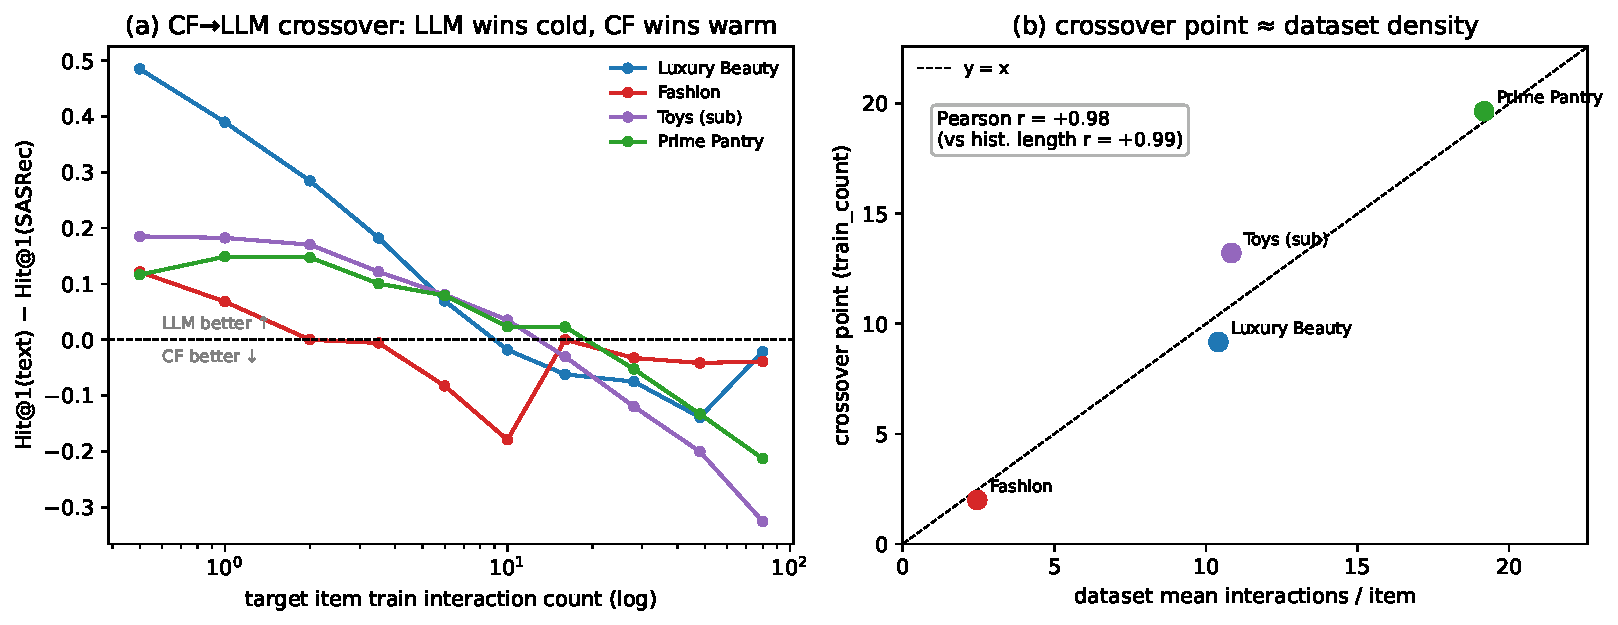
\includegraphics[width=\textwidth]{../figures/crossover_sparsity.pdf}
\caption{(a) The LLM's Hit@1 advantage over collaborative filtering vs.\ the target item's training
interaction count: positive on cold items, decaying monotonically and crossing zero (CF wins warm),
in every dataset. (b) The crossover point tracks the dataset's mean interactions per item
($r\!=\!0.98$; the dashed line is $y\!=\!x$).}
\label{fig:crossover}
\end{figure}

\begin{table}[t]
\centering
\caption{Ranking Hit@1, sliced cold/warm (seed~0). The LLM (\emph{text}) wins on cold items;
collaborative filtering (\emph{SASRec}) wins on warm items --- the crossover, in all four datasets.}
\label{tab:crossover}
\begin{tabular}{lcccc}
\toprule
 & \multicolumn{2}{c}{Cold} & \multicolumn{2}{c}{Warm} \\
\cmidrule(lr){2-3}\cmidrule(lr){4-5}
Dataset & SASRec & text & SASRec & text \\
\midrule
Luxury Beauty   & 0.169 & \textbf{0.492} & \textbf{0.710} & 0.666 \\
AMAZON\_FASHION & 0.071 & \textbf{0.158} & \textbf{0.783} & 0.725 \\
Toys \& Games   & 0.107 & \textbf{0.237} & \textbf{0.289} & 0.267 \\
Prime Pantry    & 0.026 & \textbf{0.146} & \textbf{0.332} & 0.252 \\
\bottomrule
\end{tabular}
\end{table}

% =====================================================================
\section{The Crossover Point Is Predicted by Dataset Density}
\label{sec:density}
% STYLE: Kaplan Sec.3 (present an empirical predictive relationship: state it, one clean figure,
% where it holds, honest hedge). CONTENT: FINDING_2.md.
% Crossover ~ mean interactions/item (Fig.~\ref{fig:crossover}(b)); r=0.98 (interactions/item),
% 0.99 (history length). Mechanism: CF's per-item reliability is relative to dataset density.
% Hedge: n=4.

% =====================================================================
\section{Popularity-Gated Fusion}
\label{sec:fusion}
% STYLE: Guo (Calibration) — the phenomenon implies a trivial, deployable fix (their temperature
% scaling <-> our popularity gate). CONTENT: FINDING_4.md.
% Method: z-normalise each model's candidate scores per user; fuse per candidate as
% w*z_CF + (1-w)*z_LLM with w = pop/(pop+pivot), pivot = mean interactions/item (Sec.~\ref{sec:density}).
% Result: beats BOTH pure models on Hit@1 and NDCG on all 4 (Table~\ref{tab:fusion}); naive fusion
% (RRF / equal-weight) does not. Honest nuance: Prime Pantry is CF-dominant -> pop-gate wins
% Hit@1/NDCG but pure CF wins Hit@5/10 there.

\begin{table}[t]
\centering
\caption{CF+LLM fusion (ranking, seed~0). \emph{pop-gate} is the deployable popularity-gated fusion;
\emph{oracle} routes by the true target's popularity (upper bound, not deployable). pop-gate beats
both pure models on Hit@1 and NDCG@5 on all four datasets.}
\label{tab:fusion}
\begin{tabular}{llcccc}
\toprule
Dataset & Metric & CF & text & pop-gate & oracle \\
\midrule
\multirow{2}{*}{Luxury Beauty}
 & Hit@1  & 0.501 & 0.600 & \textbf{0.622} & 0.627 \\
 & NDCG@5 & 0.611 & 0.682 & \textbf{0.718} & 0.728 \\
\midrule
\multirow{2}{*}{AMAZON\_FASHION}
 & Hit@1  & 0.246 & 0.292 & \textbf{0.308} & 0.310 \\
 & NDCG@5 & 0.314 & 0.385 & \textbf{0.405} & 0.415 \\
\midrule
\multirow{2}{*}{Toys \& Games}
 & Hit@1  & 0.206 & 0.247 & \textbf{0.266} & 0.278 \\
 & NDCG@5 & 0.347 & 0.372 & \textbf{0.414} & 0.433 \\
\midrule
\multirow{2}{*}{Prime Pantry}
 & Hit@1  & 0.254 & 0.220 & \textbf{0.286} & 0.292 \\
 & NDCG@5 & 0.428 & 0.342 & \textbf{0.436} & 0.461 \\
\bottomrule
\end{tabular}
\end{table}

% =====================================================================
\section{Discussion and Limitations}
\label{sec:discussion}
% STYLE: Dacrema (honest, evidence-first) + Kaplan caveats. CONTENT: the "Caveats" sections of the
% FINDING docs. State plainly: single seed (robustness argument = cross-dataset + monotone, not
% per-cell significance); n=4 for the density law (suggestive, not proven); 20-candidate protocol
% (metrics optimistic, relative comparisons hold); Prime Pantry Hit@5/10 nuance. Design takeaway:
% predict the crossover from density, deploy the LLM selectively / fuse by popularity.

% =====================================================================
\section{Conclusion}
\label{sec:conclusion}
% One tight paragraph: CF and LLMs are complementary along item popularity; the crossover is
% predictable from data density and exploitable by a simple popularity-gated fusion. LLMs are a
% cold-start specialist, not a general upgrade.

% ---- Bibliography ----
\bibliographystyle{splncs04}
\bibliography{refs}

\end{document}
